%!TEX root = ../main.tex
%%%%%%%%%%%%%%%%%%%%%%%%%%%%%%%%%%
% Links:
%
% Difficulty: Companies: 
%%%%%%%%%%%%%%%%%%%%%%%%%%%%%%%%%%


%\begin{figure} \centering 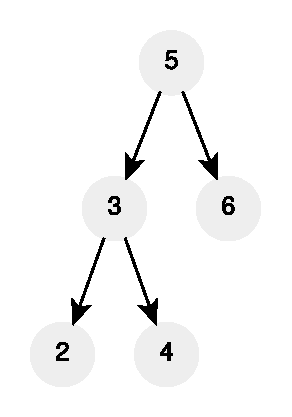
\includegraphics[width=\textwidth]{sources/decode_string/images/example1}
%   \caption[Sample short cpation]{Sample Caption}. \label{fig:decode_string:example1} \end{figure}

\chapter{Ways of decoding a message}
\label{ch:decode_string}
\section*{Introduction}
This problem resemble the problem of decoding a string encoded with the famous \textit{run-length
encoding method}(RLE)\footnote{It is a simple form of data compression in
which a stream of data is given (like the following string "AAABBCCCC") 
and the output is a sequence of	counts of consecutive data values in a row. 
(i.e. "3A2B4C").
It is a type of lossless encoding meaning that the encoding process does not lose any information in the 
original input and therefore the input data can be recovered fully and integrally.
decoded.} 

The problem discussed in this chapter is going to deal with a similar algorithm and you are asked to write a 
decode function for a string encoded with a run-length-encoding-like algorithm.


\section{Problem statement}
\begin{exercise}
\label{example:decode_string:exercice1}
Write a function that given an encoded string $s$ decodes it.
$s$ is of the form: ${k_1[d_1]k_2[d_2[ \ldots]}$ where $k$ is a positive integer and $s$ is another encoded string. 
The decoded version of $s$ is obtained by appending $d_1$ $k_1$ followed by repeating $d_2$ $k_2$ times.
 
	%example1
	\begin{example}
		\label{example:decode_string:example1}
		\hfill \\
		Given \inline{s="2[abc]3[ab]"} the function returns \inline{"abcababababcababab"}.
	\end{example}

	%example2
	\begin{example}
		\label{example:decode_string:example2}
		\hfill \\
		Given \inline{s="2[abc3[ab]]"} the function returns \inline{"abcababababcababab"}.
	\end{example}

	\begin{example}
		\hfill \\
		Given \inline{s="2[abc]3[cd]ef"} the function returns \inline{"abcabccdcdcdef"}.

	\label{ex:decode_string:example3}
	\end{example}
\end{exercise}

\section{Clarification Questions}

\begin{QandA}
	\item Is it guaranteed that $s$ is always valid?
	\begin{answered}
		\textit{Yes, $s$ contains only lower-case letters from the English alphabet, numbers and square brackets and it is valid encoded string. .}
	\end{answered}

\end{QandA}

\section{Discussion}
\label{decode_string:sec:discussion}
Let's start by noticing that this problem is really easy when
$s$ does not have any nested encoded string. If inside each of the square brackets we only find letters
then all we have to do is to replicate these letters by the associated counter and move on onto the next square brackets where we do the same. 
At the end of the process we can assemble the final answer by concatenating all the strings we obtained by the processed described above.
For instance w.r.t. the input string shown in Example \ref{example:decode_string:example1} we can decode 
\inline{2[abc]} and \inline{3[ab]} separately and obtain \inline{abcabc} and \inline{ababab}, respectively, which can then be concatenated to obtain the final answer.



\subsection{Brute-force}
\label{decode_string:sec:bruteforce}

\begin{minipage}{\linewidth}
	\lstinputlisting[language=c++, caption={Sample Caption},label=list:decode_string]{sources/decode_string/decode_string_solution1.cpp}
\end{minipage}

